\begin{kasten}
    \section*{ \hspace{0.1cm} {\color{red} \underline{RESULTS}}}
    \large{
\begin{figure}[H]
\renewcommand{\baselinestretch}{0.5}
\noindent
{\scriptsize
\begin{tabular}{c r  @{} c c }
\multicolumn{4}{c}{Weighted Performance (Multiple Datasets)} \\\hline

Rank & Treatment  & 50\% & \% Ret \\
\hline

1 & NaiveBayes & \boxplot{68.8}{18.6}{87.4}{6.7}{94.1} & 14.1 \\
2 & WeightedMeans1 & \boxplot{53.9}{18.7}{72.6}{12}{84.6} & 14.1 \\
3 & WeightedMeans0 & \boxplot{53.9}{18.7}{72.6}{12.6}{85.2} & 14.1 \\
4 & Centroid & \boxplot{48.1}{15.5}{63.6}{19.5}{83.1} & 14.1 \\
5 & HyperPipes & \boxplot{40.4}{14.5}{54.9}{22}{76.9} & 14.1 \\
6 & RemoveOutliers & \boxplot{42.4}{11}{53.4}{26.5}{79.9} & 60.2 \\
7 & OverfitRevert & \boxplot{38.1}{10.2}{48.3}{21.5}{69.8} & 66.4 \\
8 & MultiPipes & \boxplot{38.1}{9.2}{47.3}{22.7}{70.0} & 67.3 \\
9 & 5\%Alpha & \boxplot{2.4}{17.3}{19.7}{32.2}{51.9} & 88.4 \\
10 & 25\%Alpha & \boxplot{0.7}{2.8}{3.5}{29.8}{33.3} & 97.1 \\
11 & 50\%Alpha & \boxplot{0.2}{0.5}{0.7}{14.1}{14.8} & 99.3 \\



\end{tabular}
}

\end{figure}


\begin{figure}[H]
\renewcommand{\baselinestretch}{0.5}
\noindent
{\scriptsize
\begin{tabular}{c r  @{} c }
\multicolumn{3}{c}{Weighted Performance (Many Classes Datasets)} \\\hline

Rank & Treatment  & 50\% \\
\hline

1 & WeightedMeans1 & \boxplot{53.7}{16.3}{70.0}{18.9}{88.9} \\
2 & WeightedMeans0 & \boxplot{53.7}{16.3}{70.0}{18.9}{88.9}\\
3 & MultiPipes & \boxplot{53.7}{16.3}{70.0}{18.9}{88.9}\\
4 & RemoveOutliers & \boxplot{53.7}{16.1}{69.8}{19.1}{88.9} \\
5 & OverfitRevert & \boxplot{53.7}{16.1}{69.8}{19.1}{88.9} \\
6 & NaiveBayes & \boxplot{42.1}{23.2}{65.3}{18.4}{83.7} \\
7 & HyperPipes & \boxplot{21.1}{38}{59.1}{16.2}{75.3} \\
8 & Centroid & \boxplot{23.4}{34.4}{57.8}{16.4}{74.2} \\
9 & 5\%Alpha & \boxplot{33.8}{20.6}{54.4}{14.7}{69.1} \\
10 & 25\%Alpha & \boxplot{22.7}{11.1}{33.8}{24.1}{57.9} \\
11 & 50\%Alpha & \boxplot{18.2}{4.4}{22.6}{3.2}{25.8} \\



\end{tabular}
}

\end{figure}


    }

\end{kasten}

\begin{kasten}
    \section*{ \hspace{0.1cm} {\color{red} \underline{WHAT WE FOUND}}}
     \large{

	}
\begin{comment}
    \vspace{-0.5em}
    \large{
      \begin{minipage}{4.5cm}
          \begin{center}
            {\small{
            Low dynamism: $\sigma=0, \lambda=0$
            
            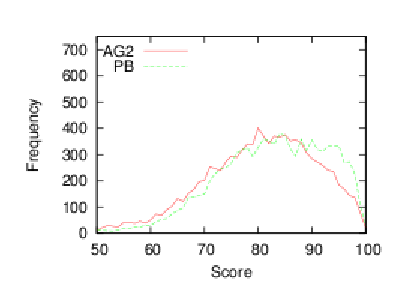
\includegraphics[width=4.5cm]{fr-v-sc-msvl.eps}
            
            Medium dynamism: $\sigma=0.15, \lambda=0.015$
            
            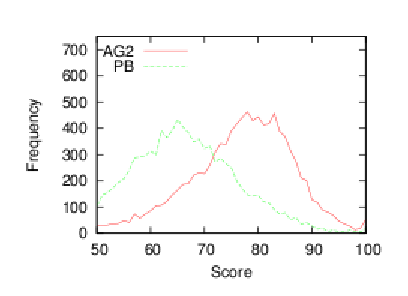
\includegraphics[width=4.5cm]{fr-v-sc-msmi.eps}
            
            High dynamism: $\sigma=2, \lambda=0.2$
            
            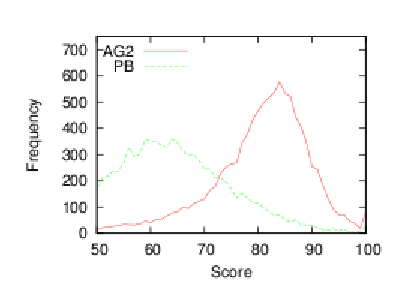
\includegraphics[width=4.5cm]{fr-v-sc-msvh.eps}
            }}
          \end{center}
      \end{minipage}
      \begin{minipage}{8.5cm}
        We ran KEYS 1000 times for each combination of {very low, medium, very high} dynamism and {plan-based, agile 2} prioritization policy. The findings are summarized in \S{RESULTS}. Several majority case effects deserve note:
        \vspace{-0.8em}
        \begin{verysmallitem}
        \item Criticality Modifier: Never chosen in more than $1\%$ of the cases.
        \item Initial Known$/$Inter-Dependency: Never chosen in $>50\%$ of the runs.
        \item Team Size: Never $<5$ team members.
        \item For Agile 2:
          \vspace{-0.7em}
          \begin{verysmallitem}
          \item Size: The smallest size was chosen in $72\%-100\%$ of the runs.
          \item Culture: The upper bins were chosen in $72\%-80\%$ of the runs where dynamism was a factor.
          \item Team Size: Should be 5 - 17 for medium and very high dynamism.
          \end{verysmallitem}
        \end{verysmallitem}

\vspace{-0.8em}
The 1000 runs of KEYS shows that many
results are very similar (e.g. all the Agile 2
          results offer nearly the same pattern). 
KEYS shows that there are two major divisions of 
its 10-dimensional space: very high criticality 
and very small team size. We ran 10,000 
simulations in the union of these two divisions
      \end{minipage}
    }

 (shown above). The median score of Agile 
2 is shows stability under changing dynamism, while 
the median score of Plan-Based falls  as dynamism increases. We see that the median score of Agile 2 is equal to or greater than the median score of Plan-Based development.

    \vspace{3mm}
    We conclude that in the general case, Agile 2 out performs Plan-Based development. Only rarely does Plan-Based out perform Agile 2.
    \vspace{-0.1em}
\end{comment}
\end{kasten}

\begin{kasten}
    \section*{ \hspace{0.1cm} {\color{red} \underline{FOR MORE INFORMATION}}}
    \vspace{-0.5em}
    \normalsize{
      Aaron Riesbeck (\url{aaron.riesbeck@gmail.com})\\
      Adam Brady (\url{adam.m.brady@gmail.com})\\
      Tim Menzies Ph.D. (\url{tim@menzies.us})\\
    }
    \vspace{-0.5em}
\end{kasten}

\begin{kasten}
    \section*{ \hspace{0.1cm} {\color{red} \underline{References}}}
    \vspace{-0.5em}
    \normalsize{
      \begin{enumerate}
      \item J. Eisenstein and R. Davis. Visual and linguistic information in gesture classification. In ICMI, pages 113-120, 2004.
      \item R. J. Larsen and M. L. Marx. An Introduction to Mathematical Statistics and Its Applications, Third Edition. Prentice Hall, 2001.
      \item I. H. Witten and E. Frank. Data Mining: Practical Machine Learning Tools and Techniques with Java Implementations. Morgan Kaufmann, 1999.
      \end{enumerate}
    }
\end{kasten}
